\documentclass[12pt,a4paper]{article}
\usepackage[utf8]{inputenc}
\usepackage[german]{babel}
\usepackage[T1]{fontenc}
\usepackage{amsmath}
\usepackage{amsfonts}
\usepackage{amssymb}
\usepackage[left=2cm,right=2cm,top=2cm,bottom=2cm]{geometry}
\usepackage{graphicx}
\usepackage{hyperref}
\usepackage{multicol}
\author{Jan Lorenz, Vincent Schnoor, Tim Zschage}
\title{Lokalisierung von Schallquellen in Unity}
\begin{document}
\maketitle
\begin{center}
Projektlink: \href{https://github.com/TheCanadians/AudioLocalization}{Audio Localization Project}
\end{center}

\section{Motivation}
Die Außenohr-Übertragungsfunktion oder Head-Related Transfer Function, kurz HRTF, ist dafür da, Sound möglichst realistisch darzustellen, indem es die Form von Außenohr, Kopf und Rumpf mit einbezieht.\\
Da die HRTF sehr individuell ist, braucht man eine gute Durchschnitts-HRTF, die für eine breite Masse funktioniert. Deshalb benötigt man in Studien zur Untersuchung von HRTFs möglichst viele Probanden um ein breites Ergebnis zu bekommen. Es ist jedoch schwierig genügend Studienteilnehmer zu finden, weshalb man eine Alternative finden muss, um nicht zwangsläufig von der Zahl der Probanden abhängig zu sein.\\
In unserem Projekt wollen wir im Rahmen einer Simulation in Unity eine Anwendung entwickeln, welche die Position einer Geräuschquelle mit höchstmöglicher Genauigkeit bestimmt, um damit die Notwendigkeit von physischen Probanden zu eliminieren.

\section{Herangehensweise}
Um eine Schallquelle anhand verschiedener Audiospuren möglichst genau lokalisieren zu können, haben wir uns mit zwei Verfahren vertraut gemacht, welche in der Realität zu diesem Zweck verwendet werden:

\subsection{Pegeldifferenzbestimmung}
Bei der Pegeldifferenzbestimmung wird der Pegel des linken Kanals und des rechten Kanals miteinander verglichen. Sind die Pegel identisch, lässt dies darauf schließen, dass sich die Audioquelle direkt vor oder direkt hinter dem Audio Listener befindet. Dreht sich der Audio Listener komplett um die eigene Achse, wird es zwei Punkte geben, an denen die Pegeldifferenzen ein Maximum haben. Dies ist das Resultat davon, dass sich die Audioquelle entweder links oder rechts vom Audio Listener befindet.\\ 
Die Pegeldifferenzbestimmung kann man auch dazu nutzen, die Elevation der Audioquelle zu bestimmen. Dazu wird nach Bestimmung des Azimuts der Audio Listener um die horizontale Achse relativ zur Audioquelle gedreht. Dies erreicht dieselbe räumliche Anordnung von Audioquelle und Audio Listener wie bei der Bestimmung des Azimuts und das obig beschriebene Verfahren kann zur Bestimmung der Elevation wiederholt werden. 

\subsubsection{Erwartung}
Mit diesem Lösungsansatz erwarten wir eine simplere und verlässlichere Umsetzung, die jedoch eine geringere Lokalisationsgeschwindigkeit mit sich bringt.
Unsere Umsetzung soll für eine gegebene Rotationsposition den linken und rechten Kanal vergleichen und sich anschließend in Richtung des lauteren Kanals bewegen. Anschließend wird der Vorgang so lange fortgeführt, bis der vorher leisere Kanal zum lauteren Kanal wird, denn dies bedeutet, dass die Audioquelle direkt vor dem Audio Listener liegt.


\subsection{Interaurale Kreuzkorrelation}
Bei der Interauralen Kreuzkorrelation können die Interaurale Leveldifferenz (ILD) und die Interaurale Zeitdifferenz (ITD) für die Bestimmung des Azimuts der Audioquelle genutzt werden \cite{Fall}.\\
Die ILD ist die wahrgenommene  frequenzabhängige Pegeldifferenz in dB zwischen beiden Ohren.\\ 
Die ITD ist die frequenzabhängige zeitliche Phasenverschiebung \(\omega\) zwischen beiden Ohren.\\
ITD liefert genauere Ergebnisse für niedrige Frequenzen, da Phasenverschiebungen genauer zu identifizieren sind. ILD liefert genauere Ergebnisse bei hohen Frequenzen, deren Wellenlänge wesentlich kleiner als der Abstand zwischen den Ohren ist.\\
Da beide Verfahren der Bestimmung des Azimuts dienen, können sie gleichzeitig verwendet werden, um die Azimutbestimmung zu verbessern \cite{Rasp}.

\subsubsection{Erwartung}
Da die Interaurale Kreuzkorrelation einen Zusammenhang zwischen beiden Ohren herstellt, erwarten wir eine sofortige und genaue Bestimmung des Azimuts. Diese sollte nicht über eine sukzessive Annäherung erfolgen, sondern eine direkte Angabe des Winkels bei jeder gegebenen Position liefern.

\subsection{Head-related Transfer Function (HRTF)}
Die Head-related transfer function function (HRTF) ist eine Transferfunktion, welche beschreibt, wie ein Hörereignis von einem individuellen Kopf und dessen Ohrmuscheln verändert wird, bevor es in den Gehörgang tritt.\\
Der Einsatz einer HRTF wirkt sich positiv auf die Lokalisationsfähigkeit einer Person aus.

\section{Umsetzung}
\subsection{Unity-Szene}
Um unsere Anwendung testen zu können, musste eine Unity-Szene erstellt werden, in welcher folgende Components benötigt werden: Audio Source und Audio Listener. Auf der Audio Source liegt ein Spawn-Skript, welches bestimmt, an welcher zufälligen Position in einem Kreis um den Audio Listener herum die Audio Source beim Start der Simulation erscheint (siehe Bild 2). Dabei muss das Audio Source-Component folgendermaßen konfiguriert sein:

\begin{figure}[h!]
\centering
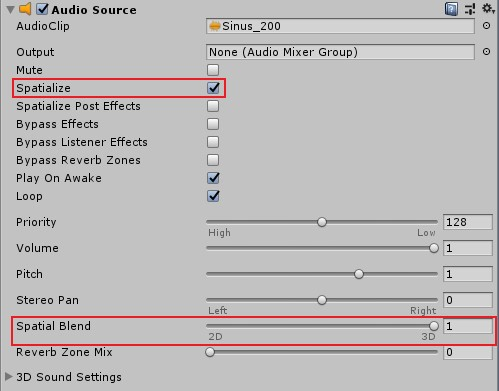
\includegraphics[scale=0.6]{setup2}
\caption{Bild 1: Audio Source-Konfiguration}
\end{figure}

Auf dem Audio Listener muss das Skript liegen, welches zur Lokalisation der Audioquelle dient.\\
Weiterhin muss in den Projekteinstellungen, im Reiter Audio, ein Spatializer-Plugin (HRTF) angegeben werden.\\
In dem Projekt wurden verschiedene Spatializer verwendet. Die Unity Engine stellt mit dem „Windows Mixed Reality Package und dem „Oculus Desktop Package”, zwei installierbare Pakete nativ zur Verfügung. Zusätzlich wurde der „Steam Audio Spatializer“ als Drittanbieter Software eingebunden. Steam Audio ist ein Audio Plugin, das seit 2017 von der Firma Valve angeboten wird und darauf abzielt, den Sound in Videospielen so realistisch wie möglich klingen zu lassen.\\

Wir ließen die Anwendung mit den drei Spatializern, sowie ein weiteres Mal ohne Spatializer, durchlaufen und die daraus resultierenden Daten, geschätzter Winkel, tatsächlicher Winkel und Abweichung wurden in einem Spreadsheet festgehalten.

\subsection{Skript}
Das Skript für die Lokalisation der Audioquelle geht folgende Schritte durch:
\begin{enumerate}
\item Auslesen der Spannungswerte der einzelnen Kanäle und Umwandlung in Pegel (dB)
\item Vergleich der Pegelwerte beider Kanäle
\item Rotation in Richtung des lauteren Kanals
\item Prüfung, in welche Richtung sich der Audio Listener im letzten Schritt bewegt hat
\item Sobald die Richtung sich geändert hat, wurde der Azimut der Audioquelle bestimmt
\end{enumerate}

\begin{figure}[h!]
\centering
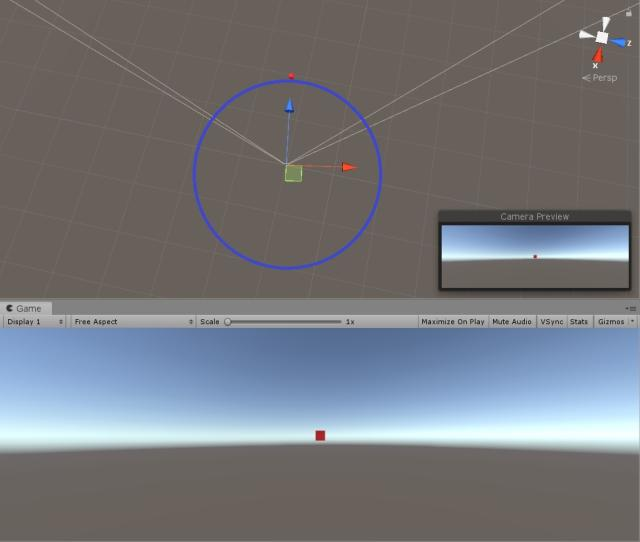
\includegraphics[scale=0.5]{setup1}
\caption{Bild 2: Audioquelle (rot) dreht befindet sich auf einer randomisierten Position auf dem Kreis (blau) um den Audio Listener innerhalb des Kreises}
\end{figure}

\subsection{Wahl der Audioclips}
Um die Funktionalität für verschiedene Audioclips zu verifizieren, wurden sowohl Mono- als auch Stereo-Clips verwendet.\\ 
Die Frequenzabhängigkeit der Interauralen Kreuzkorrelation wird geprüft, indem Sinussignale mit mehreren Frequenzen verwendet werden.\\ 
Ebenso werden Audioclips mit rosa Rauschen und weißem Rauschen, Musik und Sprache geprüft.\\

Verwendet wurden:
\begin{multicols}{2}
\begin{itemize}
\item Rosa Rauschen
\item Weißes Rauschen
\item Sinus 200 Hz
\item Sinus 1000 Hz
\item Sinus 2000 Hz
\item Sinus 3200 Hz (Mono)
\item Sinus 3200 Hz (Stereo)
\item Sprache (Stereo)
\item Orchesteraufnahme (Stereo)
\item[\vspace{\fill}]
\end{itemize}
\end{multicols}

Die Auswahl der Sinusfrequenzen leitet sich aus der Wellenlänge ab. Basierend auf einem wirksamen Ohrabstand von 21 cm leitet sich eine Frequenz von rund 1600 Hz ab. Demnach wählen wir Frequenzen über und unter 1600 Hz aus, um zu prüfen, ob unterschiedliche Ergebnisse bei der Interauralen Kreuzkorrelation entstehen.\\

Die Unterscheidung von Mono- und Stereospuren wurde vorgenommen, um zu prüfen, ob die Unity-Engine diese anders verarbeitet und andere Ergebnisse daraus resultieren. 

\section{Durchführung des Versuchs}

\section{Resultate}
\subsection{Kreuzkorrelationsfunktion}
Bei dem Versuch, den Azimut mit der interauralen Kreuzkorrelation zu bestimmen, stellte sich heraus, dass die Unity-Engine Audiosignale zeitunabhängig berechnet. Eine Lokalisation mit der interauralen Kreuzkorrelation war deshalb nicht möglich, da diese ausschließlich zeitabhängig arbeitet.

\subsection{Pegeldifferenz}
Das Lokalisieren von den Audioquellen hat mit den verschiedenen Spatializern durchgehend gut funktioniert. Alle Spatializer schafften es, die Winkeldifferenz zwischen tatsächlicher Position und geschätzter Position in einem kleinen Bereich, mit einer unerheblichen Zahl an Ausreißern, zu halten.\\

Mit der MS HRTF lag die Winkeldifferenz beispielsweise meistens zwischen -19° und 9° und bei Steam Audio zwischen -7° und 12°. Besonders gut funktionierten „Speech“ und „Symphony Sounds“. Nur bei einem Sinuston von 200Hz konnte fast kein  Spatializer die Quelle genau orten. Mit einem Fehlerbereich von -4° bis 8° war der Oculus Spatializer der einzige, der die Quelle bei 200Hz ziemlich genau orten konnte. Die gemessenen Werte lassen darauf schließen, dass eine Soundquelle mit 200Hz mit dem Einsatz von Spatializern schwer zu lokalisieren ist.\\

Die Abweichungen bei 200Hz waren zwar unter den Spatializer recht weit auseinander aber die Werte lagen dennoch ziemlich konstant beieinander. Der MS HRTF Spatializer wies beispielsweise eine Abweichung im Bereich -51° bis -54° und der Native Oculus Spatializer im Bereich -4° bis 8° auf. Lediglich der Steam Audio Spatializer war ziemlich ungenau mit Abweichungen im Bereich von -172° bis 167°.\\

\begin{figure}[h!]
\centering
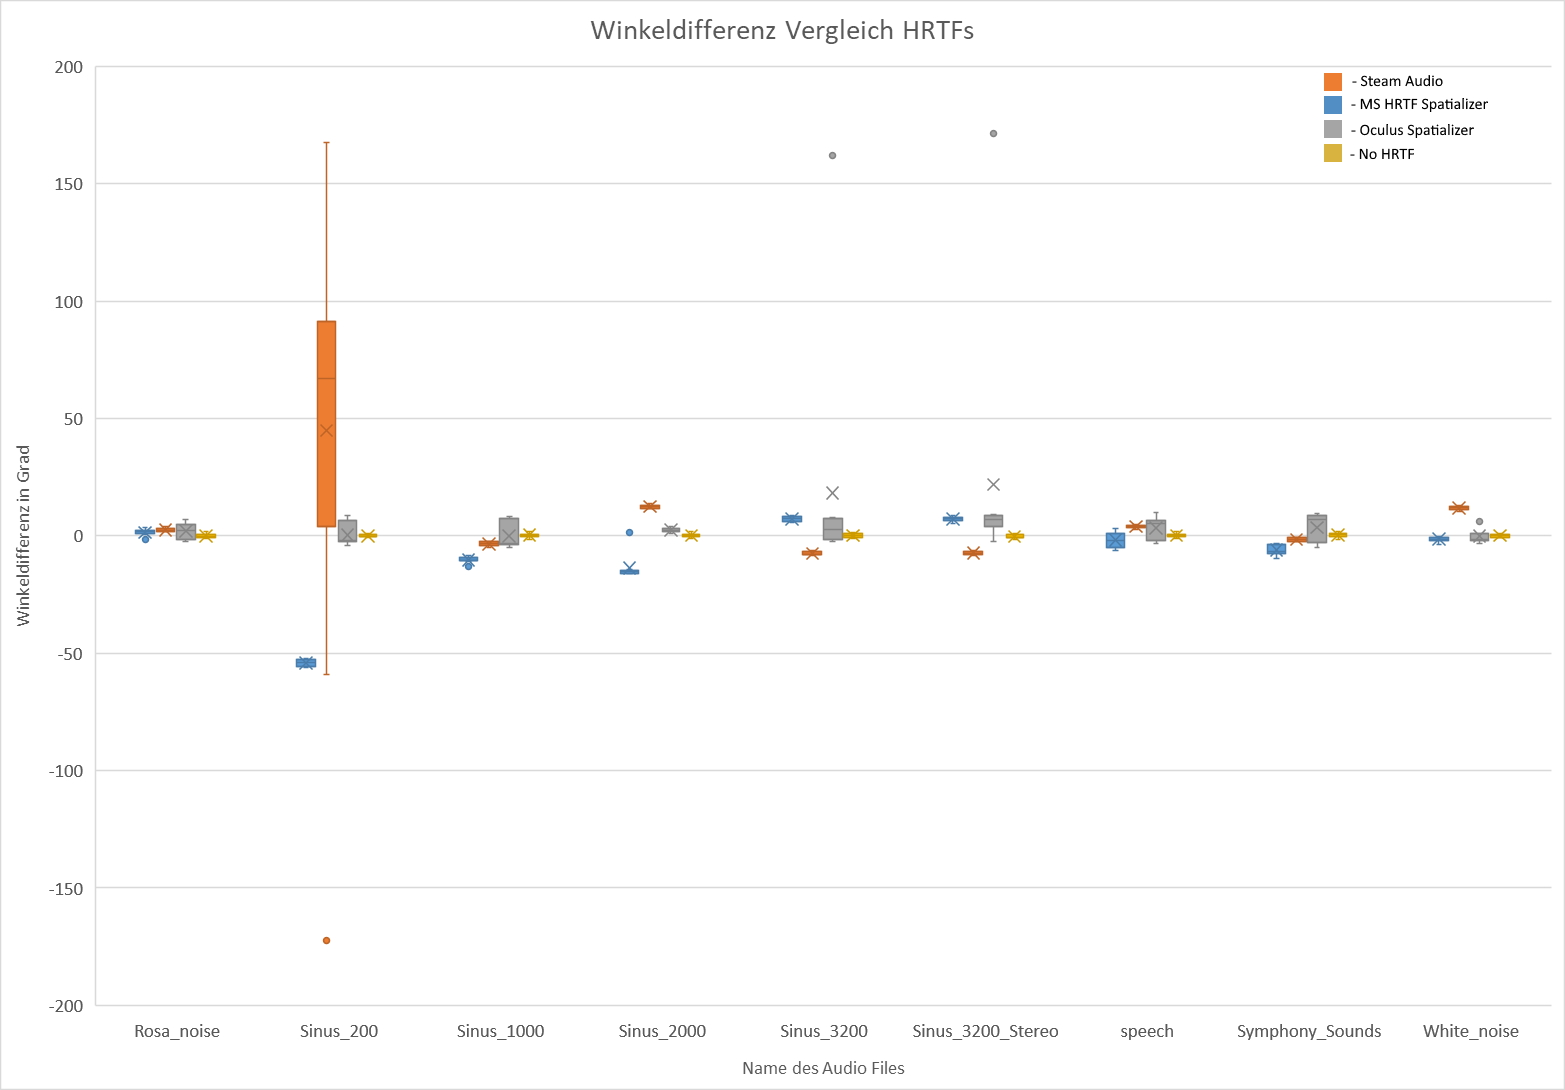
\includegraphics[scale=0.4]{Vergleich_HRTFs}
\caption{Bild 3: Vergleich der verschiedenen HRTFs}
\end{figure}

Man erkennt in der Abbildung, dass das Lokalisieren von Audioquellen ohne Spatializer anhand der Pegeldifferenzbestimmung sehr genau ist. Die größte Abweichung wurde hier mit 1,9° gemessen.



\bibliographystyle{plain}
\bibliography{sources}
\end{document}